%============================================================================
% LaTeX File
% Daniel J. Greenhoe
%============================================================================
%======================================
\chapter{Some Probability Density Functions}
%======================================
%=======================================
\section{Discrete distributions}
%=======================================
\begin{figure}[t]
\centering
\begin{tabular}{*{11}{c}}
  $\scriptstyle \psp\setn{ 2}=\frac{1}{36}$ &
  $\scriptstyle \psp\setn{ 3}=\frac{2}{36}$ &
  $\scriptstyle \psp\setn{ 4}=\frac{3}{36}$ &
  $\scriptstyle \psp\setn{ 5}=\frac{4}{36}$ &
  $\scriptstyle \psp\setn{ 6}=\frac{5}{36}$ &
  $\scriptstyle \psp\setn{ 7}=\frac{6}{36}$ &
  $\scriptstyle \psp\setn{ 8}=\frac{5}{36}$ &
  $\scriptstyle \psp\setn{ 8}=\frac{4}{36}$ &
  $\scriptstyle \psp\setn{10}=\frac{3}{36}$ &
  $\scriptstyle \psp\setn{11}=\frac{2}{36}$ &
  $\scriptstyle \psp\setn{12}=\frac{1}{36}$
  \\                  &                  &                  &                  &                  & \diceF\diceA &                  &                  &                  &                  &
  \\                  &                  &                  &                  & \diceE\diceA & \diceE\diceB & \diceF\diceB &                  &                  &                  &
  \\                  &                  &                  & \diceD\diceA & \diceD\diceB & \diceD\diceC & \diceE\diceC & \diceF\diceC &                  &                  &
  \\                  &                  & \diceC\diceA & \diceC\diceB & \diceC\diceC & \diceC\diceD & \diceD\diceD & \diceE\diceD & \diceF\diceD &                  &
  \\                  & \diceB\diceA & \diceB\diceB & \diceB\diceC & \diceB\diceD & \diceB\diceE & \diceC\diceE & \diceD\diceE & \diceE\diceE & \diceF\diceE &
  \\ \diceA\diceA & \diceA\diceB & \diceA\diceC & \diceA\diceD & \diceA\diceE & \diceA\diceF & \diceB\diceF & \diceC\diceF & \diceD\diceF & \diceE\diceF & \diceF\diceF
\end{tabular}
  \caption{
    Probability distribution for two dice (see \prefp{ex:two_dice})
    \label{fig:two_dice}
    }
\end{figure}
%---------------------------------------
\begin{example}
\footnote{
  \citer{osgood}
  }
\label{ex:two_dice}
%---------------------------------------
Suppose we throw two ``fair" dice and want to know the probabilities of their sum.
Let $\rvX$ represent the sum  of the face values of the two dice.
The resulting probability distribution is illustrated in \prefpp{fig:two_dice}
and has probability space as follows:

\exbox{\begin{array}{ll}
  \pso &= \setn{\text{\diceA\diceA,\; \diceA\diceB,\; \diceA\diceC,\;\ldots,\;\diceF\diceF} }
  \\
  \pse &= \left\{ \pset{\set{X=n}{n=2,3,\ldots,10,11,\text{ or } 12}} \right\}
  \\
  \psp(e) &= \frac{1}{36} \seto{e}
\end{array}}

\end{example}

%=======================================
\section{Continuous distributions}
%=======================================
%=======================================
\subsection{Uniform distribution}
%=======================================
%---------------------------------------
\begin{definition}
\label{def:uniform}
%---------------------------------------
The \fnctd{uniform distribution} $\ppx(x)$ is defined as
\defbox{
  \ppx(x) \eqd \brb{\begin{array}{lM}
                      1  & for $0< x \le 1$\\
                      0  & otherwise
                    \end{array}}
  }
\end{definition}

Note that although ``simple" in form, in light of \thme{Wold's Theorem}, the
value of the \fncte{uniform distribution} should \emph{not} be taken lightly.

%=======================================
\subsection{Gaussian distribution}
\index{Gaussian distribution}
\index{normal distribution}
%=======================================
\qboxnpqt
  {Bernard A. Lippmann as told by Henri Poincar\'e
  \index{Lippmann, Bernard A.} \index{Poincar\'e, Henri}
  \index{quotes!Lippmann, Bernard A.} \index{quotes!Poincar\'e, Henri}
   \footnotemark
  }
  {../common/people/poincare.jpg}
  {Tout le monde y croit cependant, me disait un jour M. Lippmann,
   car les exp\'erimentateurs s'irnaginent q\`ue c'est un th\'eor\`eme
   de math\'ematiques, et les math\'ematiciens que c'est un fait
   exp\'erimental.}
  {Everyone believes in it [(the normal distribution)] however,
   said to me one day Mr. Lippmann, because the experimenters imagine that
   it is a theorem of mathematics,
   and mathematicians that it is an experimental fact.}
  \citetblt{
    quote:       & \citerp{poincare_calc_prob}{171} \\
    translation: & assisted by \href{http://translate.google.com/}{Google Translate} \\
    image:       &
    }

\begin{figure}[ht]
   \begin{center}
   \includegraphics[height=8cm, width=12cm, clip=]{../common/pdf_norm.eps}
   \end{center}
\caption{
  Gaussian pdf with $\mu=0$ and $\sigma\in[0.1,2]$.
  \label{fig:pdf_norm}
  }
\end{figure}

%---------------------------------------
\begin{definition}
%---------------------------------------
\defbox{\begin{array}{c>{\ds}rc>{\ds}l}
  \mc{4}{M}{The \fnctd{Gaussian distribution} (or \fnctd{normal distribution}) has pdf}
    \\& \ppx(x) &\eqd& \frac{1}{\sqrt{2\pi\sigma^2}}e^{\frac{-(x-\mu)^2}{2\sigma^2}}
    \\
  \mc{4}{M}{A random variable $\rvX$ with this distribution is denoted}
    \\& \rvX &\sim& \pN{\mu}{\sigma^2}
    \\
  \mc{4}{M}{The function $\fQ(x)$ is defined as the area under a Gaussian PDF}\\
  \mc{4}{M}{with zero mean and variance equal to one from $x$ to infinity such that}
    \\& \fQ(x) &\eqd& \frac{1}{\sqrt{2\pi}} \int_x^\infty e^{\frac{-u^2}{2}} \du
\end{array}}
\end{definition}

%=======================================
\subsection{Gamma distribution}
%=======================================
%---------------------------------------
\begin{definition}
\label{def:Gamma(b)}
\index{gamma function}
\index{$\Gamma(b)$}
\footnote{
  \citerp{papoulis}{79},
  \citerp{ross}{222}
  }
%---------------------------------------
Let $b\in\R$. The \fnctd{gamma function} $\Gamma(b)$ is
\defbox{ \Gamma(b) \eqd \int_0^\infty x^{b-1} e^{-x} \dx  }
\end{definition}

%---------------------------------------
\begin{proposition}
\footnote{
  \citerp{ross}{223}
  }
%---------------------------------------
Let $b\in\R$ and $n\in\Zp$.
\propbox{\begin{array}{rcl}
  \Gamma(b) &=& (b-1)\Gamma(b-1)  \\
  \Gamma(n) &=& (n-1)!
  \end{array}}
\end{proposition}
\begin{proof}
Let
\[\begin{array}{rcl@{\hspace{2cm}}rcl}
  u   &=& x^{b-1}   & \du &=& (b-1)x^{b-1} \dx \\
  \dv &=& e^{-x}\dx & v   &=& -e^{-x}
\end{array}\]

\begin{eqnarray*}
  \Gamma(b)
    &\eqd& \int_0^\infty x^{b-1} e^{-x} \dx
  \\&=&    \int_{x=0}^\infty u \dv
  \\&=&    uv|_{x=0}^\infty - \int_{x=0}^\infty v \du
  \\&=&    -x^{b-1} e^{-x}|_{x=0}^\infty + (b-1)\int_{x=0}^\infty e^{-x} x^{b-1}\dx
  \\&=&    (-0+0) + (b-1)\Gamma(b-1)
\end{eqnarray*}

Note that
  \[ \Gamma(1)
       = \int_0^\infty x^{1-1} e^{-x} \dx
       = \int_0^\infty e^{-x} \dx
       = \left. -e^{-x} \right|_0^\infty
       = -0 + 1
       = 1
  \]
\begin{eqnarray*}
  \Gamma(n)
    &=& (n-1)\Gamma(n-1)
  \\&=& (n-1)(n-2)\Gamma(n-2)
  \\&=& (n-1)(n-2)(n-3)\Gamma(n-3)
  \\&\vdots&
  \\&=& (n-1)(n-2)(n-3)\cdots(1)\Gamma(1)
  \\&=& (n-1)(n-2)(n-3)\cdots(1)
  \\&\eqd& (n-1)!
\end{eqnarray*}
\end{proof}

%---------------------------------------
\begin{definition}
%---------------------------------------
A \fnctd{Gamma distribution} $(b,\lambda)$ has pdf
\defbox{ \ppx(x) \eqd \frac{\lambda}{\Gamma(b)} e^{-\lambda x}(\lambda x)^{b-1} }
\end{definition}

%---------------------------------------
\begin{theorem}
\label{thm:Gamma_X+Y}
\footnote{
  \citerp{ross}{266}
  }
%---------------------------------------
Let $\rvX$ and $\rvY$ be \fncte{random variable}s on a \structe{probability space} $\ps$.
\thmbox{
  \brb{\begin{array}{FMD}
      (A).& $\rvX$ and $\rvY$ are \prope{independent}                  & and
    \\(B).& $\rvX$ has \prope{Gamma distribution} $\opair{a}{\lambda}$ & and
    \\(C).& $\rvY$ has \prope{Gamma distribution} $\opair{b}{\lambda}$ & and
    \\(D).& $\rvZ\eqd\rvX+\rvY$
  \end{array}}
  \implies
  \brb{\begin{array}{M}
    $\rvZ$ has Gamma distribution\\
    $\opair{a+b}{\lambda}$.
  \end{array}}
  }
\end{theorem}
\begin{proof}
\begin{align*}
  \ppz(z)
    &= \ppx(z)\conv\ppy(z)
  \\&= \int_{u\in\R} \ppx(u)\ppy(z-u) \du
    && \text{by definition of \ope{convolution}}
    && \text{\xref{def:conv}}
  \\&= \int_0^z
       \frac{1}{\Gamma(a)}\lambda e^{-\lambda u}(\lambda u)^{a-1}
       \frac{1}{\Gamma(b)}\lambda e^{-\lambda(z-u)}(\lambda(z-u))^{b-1}
       \du
  \\&= \frac{1}{\Gamma(a)}\frac{1}{\Gamma(b)}e^{-\lambda z}\lambda^{1+1+a-1+b-1}
       \int_0^z  u^{a-1}(z-u)^{b-1}  \du
  \\&= \frac{1}{\Gamma(a)}\frac{1}{\Gamma(b)}\lambda e^{-\lambda z}\lambda^{a+b-1}
       \int_0^1  (vz)^{a-1}(z-vz)^{b-1}  z\dv
  \\&= \frac{1}{\Gamma(a)}\frac{1}{\Gamma(b)}\lambda e^{-\lambda z}\lambda^{a+b-1}
       z^{a-1+b-1+1}
       \int_0^1  v^{a-1}(1-v)^{b-1}  \dv
  \\&= \brs{
       \frac{1}{\Gamma(a)}\frac{1}{\Gamma(b)}
       \int_0^1  v^{a-1}(1-v)^{b-1}  \dv
       }
       \lambda e^{-\lambda z}(\lambda z)^{a+b-1}
  \\&= C\lambda e^{-\lambda z}(\lambda z)^{a+b-1}
    && \text{where $C$ is some constant}
  \\&= \frac{\lambda}{\Gamma(a+b)} e^{-\lambda z}(\lambda z)^{a+b-1}
    &&\mathrlap{\text{$C$ must be the value that makes $\int_z\ppz(z)=1$}}
\\\implies & \text{$\ppz(z)$ is a $(a+b,\lambda)$ Gamma distribution}
\end{align*}
\end{proof}

%=======================================
\subsection{Chi-squared distributions}
%=======================================
%---------------------------------------
\begin{definition}
\label{def:pdf_chi}
\index{Chi-squared distribution}
\footnote{
  \citerp{proakis}{41},
  \citerpgc{papoulis1990}{219}{0137116985}{7-4 Special Distributions of Statistics, (7-78)}
  }
%---------------------------------------
Let $\pp(x)$ be a \fncte{probability density function} on a \structe{probability space} $\ps$.
\defboxt{
  $\pp(x)$ is a \fnctd{chi-square distribution} if
  \\\indentx$\ds
    \pp(x) \eqd 
    \brb{\begin{array}{>{\ds}lM}
      0                                                            &  if $x<   0$ \\
      \frac{1}{\sqrt{2\pi\sigma^2x}}\exp\brs{-\frac{x}{2\sigma^2}} &  if $x\ge 0$
    \end{array}}$
    \qquad
    for $\sigma>0$
  }
\end{definition}

%A random variable $\rvY$ with \fncte{chi-squared distribution} is equivalent
%to the square of random variable with zero-mean Gaussian distribution.
%Thus if you wanted to generate a random value with chi-square distribution,
%you could simply square the output of a Gaussian noise generator.
%---------------------------------------
\begin{theorem}
\index{chi-squared distribution}
\index{Gamma distribution}
\label{thm:Gamma=X^2}
\footnote{
  \citerp{ross}{267}
  }
%---------------------------------------
\mbox{}\\
\thmboxt{
  The following distributions are equivalent:
  \\\indentx$\begin{array}{FMD}
      (1).& chi-squared distribution                                            & and
    \\(2).& distribution of $\rvX^2$ where $\rvX\sim\pN{0}{\sigma^2}$           & and
    \\(3).& Gamma distribution $\left(\frac{1}{2},\frac{1}{2\sigma^2} \right)$  &
  \end{array}$
  }
\end{theorem}
\begin{proof}
\begin{enumerate}

\item Proof that $\rvX^2$ has chi-squared distribution:
\begin{align*}
  \ppy(y)
    &= \left.\left.\frac{1}{2\sqrt{y}}\right[
       \ppx(-\sqrt{y}) + \ppx( \sqrt{y}) \right]
    && \text{by \prefp{cor:YX2}}
  \\&= \left.\left.\frac{1}{2\sqrt{y}}\right[
       \frac{1}{\sqrt{2\pi\sigma^2}} \exp{-\frac{(-\sqrt{y}-0)^2}{2\sigma^2}}+
       \frac{1}{\sqrt{2\pi\sigma^2}} \exp{-\frac{(+\sqrt{y}-0)^2}{2\sigma^2}}
       \right]
  \\&= \left.\left.\frac{1}{2\sqrt{y}}\right[
       2\frac{1}{\sqrt{2\pi\sigma^2}} \exp{-\frac{y}{2\sigma^2}}+
       \right]
  \\&= \frac{1}{\sqrt{2\pi \sigma^2 y}} \exp{-\frac{y}{2\sigma^2}}
\end{align*}

\item Proof that chi-distribution is a Gamma distribution $(b,\lambda)$:
\begin{align*}
  b &\eqd& \frac{1}{2} \\
  \lambda &\eqd \frac{1}{2\sigma^2} \\
\\
  \frac{1}{\sqrt{2\pi\sigma^2y}}\exp{-\frac{y}{2\sigma^2}}
    &= \frac{1}{\sqrt{\pi}}\lambda^{1/2} \lambda^{1/2} (\lambda y)^{-1/2} e^{-\lambda y}
  \\&= \frac{\lambda}{\sqrt{\pi}} (\lambda y)^{b-1} e^{-\lambda y}
\end{align*}

\end{enumerate}
\end{proof}

%---------------------------------------
\begin{definition}
\index{Chi-squared distribution with $n$ degrees of freedom}
\footnote{
  \citerp{proakis}{41}
  }
%---------------------------------------
The \fnctd{Chi-squared distribution with $n$ degrees of freedom} has pdf
\defbox{
  \ppy(y) \eqd \left\{\begin{array}{ll}
    0 &:y<0 \\ \ds
    \frac{1}{2\sigma^2\Gamma(n/2)}
               \left(\frac{y}{2\sigma^2}\right)^{\frac{n}{2}-1}
               \exp{-\frac{y}{2\sigma^2}}
    &:y\ge 0
    \end{array}\right.
  }
\end{definition}

%---------------------------------------
\begin{theorem}
\index{chi-squared distribution with $n$ degrees of freedom}
\index{Gamma distribution}
\footnote{
  \citerp{ross}{267}
  }
%---------------------------------------
The following distributions are equivalent:
\begin{enumerate}
  \item chi-squared distribution with $n$ degrees of freedom
  \item the distribution of $\ds \sum_{k=1}^n X_k^2$ where
        $\set{X_k}{X_k\sim\pN{0}{\sigma^2}, k=1,2,\ldots,n}$
        are independent random variables.
  \item Gamma distribution $\left(\frac{n}{2}, \frac{1}{2\sigma^2} \right)$.
\end{enumerate}
\end{theorem}
\begin{proof}
\begin{enumerate}
\item Prove chi-squared distribution with $n$ degrees of freedom is the
      Gamma distribution $\left(\frac{n}{2}, \frac{1}{2\sigma^2} \right)$:
  \begin{eqnarray*}
    \lambda &\eqd& \frac{1}{2\sigma^2} \\
    b       &\eqd& \frac{1}{2} \\
    \frac{1}{2\sigma^2\Gamma(n/2)}
                 \left(\frac{y}{2\sigma^2}\right)^{\frac{n}{2}-1}
                 \exp{-\frac{y}{2\sigma^2}}
      &=& \frac{\lambda}{\Gamma(nb)}
          \left(\lambda y \right)^{nb-1}
          \exp{-\lambda y}
  \end{eqnarray*}

\item Prove $\sum_{k=1}^n X^2$ is Gamma $\left(\frac{n}{2}, \frac{1}{2\sigma^2} \right)$:
  \begin{enumerate}
    \item By Theorem~\ref{thm:Gamma=X^2}, $\rvX_k$ has Gamma distribution
          $\left(\frac{1}{2}, \frac{1}{2\sigma^2} \right)$.
    \item By Theorem~\ref{thm:Gamma_X+Y}, $\sum_{k=1}^n X_k^2$ has
          distribution $\left(\frac{n}{2}, \frac{1}{2\sigma^2} \right)$.
  \end{enumerate}
\end{enumerate}
\end{proof}

%---------------------------------------
\begin{definition}
\index{Noncentral chi-square distribution}
\footnote{
  \citerp{proakis}{42}
  }
%---------------------------------------
A \fnctd{noncentral chi-square distribution} $(\mu,\sigma^2)$
has pdf
\defbox{
  \ppy(y)
  = \frac{1}{\sqrt{2\pi\sigma^2y}} \exp{\frac{y+\mu^2 }{-2\sigma^2}}
          \cosh{\frac{ \mu\sqrt{y}}{\sigma^2}}
  }
\end{definition}

%---------------------------------------
\begin{theorem}
%---------------------------------------
\thmboxt{
  The following distributions are equivalent:
  \\\qquad$\begin{array}{FM}
    (1).& \fncte{non-central chi-squared distribution} $(\mu,\sigma^2)$\\
    (2).& distribution of $\rvX^2$ where $\rvX\sim\pN{\mu}{\sigma^2}$
  \end{array}$
  }
\end{theorem}
\begin{proof}
\begin{enumerate}
\item Proof that $\rvY=X^2$ has a non-central chi-squared distribution:
\begin{align*}
  \ppy(y)
    &= \left.\left.\frac{1}{2\sqrt{y}}\right[
       \ppx(-\sqrt{y}) + \ppx( \sqrt{y}) \right]
    \qquad\text{by \prefp{cor:YX2}}
  \\&= \left.\left.\frac{1}{2\sqrt{y}}\right[
       \frac{1}{\sqrt{2\pi\sigma^2}} \exp{-\frac{(-\sqrt{y}-\mu)^2}{2\sigma^2}}+
       \frac{1}{\sqrt{2\pi\sigma^2}} \exp{-\frac{(+\sqrt{y}-\mu)^2}{2\sigma^2}}
       \right]
  \\&= \left.\left.\frac{1}{2\sqrt{y}}\right[
       \frac{1}{\sqrt{2\pi\sigma^2}} \exp{-\frac{y+\mu^2 }{2\sigma^2}} \exp{\frac{-2\mu\sqrt{y}}{2\sigma^2}}+
       \frac{1}{\sqrt{2\pi\sigma^2}} \exp{-\frac{y+\mu^2 }{2\sigma^2}} \exp{\frac{ 2\mu\sqrt{y}}{2\sigma^2}}
       \right]
  \\&= \frac{1}{\sqrt{2\pi\sigma^2y}} \exp{-\frac{y+\mu^2 }{2\sigma^2}}
       \frac{1}{2}
       \left[
         \exp{\frac{ 2\mu\sqrt{y}}{2\sigma^2}} +
         \exp{\frac{-2\mu\sqrt{y}}{2\sigma^2}}
       \right]
  \\&= \frac{1}{\sqrt{2\pi\sigma^2y}} \exp{\frac{y+\mu^2 }{-2\sigma^2}}
         \cosh{\frac{ \mu\sqrt{y}}{\sigma^2}}
\end{align*}
\end{enumerate}
\end{proof}

%---------------------------------------
\begin{definition}
\footnote{
  \citerp{proakis}{43}
  }
%---------------------------------------
The \fnctd{$\alpha$th-order modified Bessel function of the first kind}
$I_\alpha(x)$ is
\defbox{
  I_\alpha(x) = \sum_{k=0}^\infty
  \frac{1}{k!\Gamma(\alpha+k+1)} \left(\frac{x}{2}\right)^{\alpha+2k}
  }
\end{definition}

%---------------------------------------
\begin{definition}
\footnote{
  \citerp{proakis}{43}
  }
%---------------------------------------
The \fnctd{noncentral chi-square with $n$-degrees of freedom} distribution has
pdf
\defbox{
  \ppy(y) =
  \frac{1}{2\sigma^2}
  \left(\frac{y}{s^2}\right)^\frac{n-2}{4}
  \exp{\frac{y+s^2}{-2\sigma^2}}
  I_{n/2-1}\left(\sqrt{y}\frac{s}{\sigma^2}\right)
  \hspace{1cm}\mbox{where }
  s^2 \eqd \sum_{k=1}^n \mu_k^2
  }
\end{definition}

%=======================================
\subsection{Radial distributions}
%=======================================
%---------------------------------------
\begin{definition}
\index{Rayleigh distribution}
\footnote{
  \citerp{proakis}{44}
  }
%---------------------------------------
The \fnctd{Rayleigh distribution} is the pdf
\defbox{
  \ppr(r) = \left\{\begin{array}{l@{\hspace{4ex}\mbox{for}\hspace{4ex}}l}
  0 & r<0 \\
  \frac{r}{\sigma^2}\exp{-\frac{r^2}{2\sigma^2}}
  & r\ge 0
  \end{array}\right.
  }
\end{definition}

Note that by Proposition~\ref{prop:XY->RT_n},
this distribution is equivalent to the distribution of
$R=\sqrt{X^2+Y^2}$ where $\rvX$ and $\rvY$ are independent random variables
each with distribution $\pN{0}{\sigma^2}$.

%---------------------------------------
\begin{definition}
\index{Rice distribution}
\footnote{
  \citerp{proakis}{46}
  }
%---------------------------------------
The \fnctd{Rice distribution} is the pdf
\defbox{
  \ppr(r) = \left\{\begin{array}{l@{\hspace{4ex}\mbox{for}\hspace{4ex}}l}
  0 & r<0 \\
  \frac{r}{\sigma^2}\exp{\frac{r^2+s^2}{-2\sigma^2}}
  I_o\left(\frac{rs}{\sigma^2}\right)
  & r\ge 0
  \end{array}\right.
  }
\end{definition}

%%=======================================
%\subsection{Nakagami $m$-distribution}
%\index{Nakagami $m$-distribution}
%\citep{proakis}{47}
%%=======================================

%=======================================
\section{Joint Gaussian distributions}
%=======================================
\begin{figure}
\begin{tabular}{*{4}{c}}
  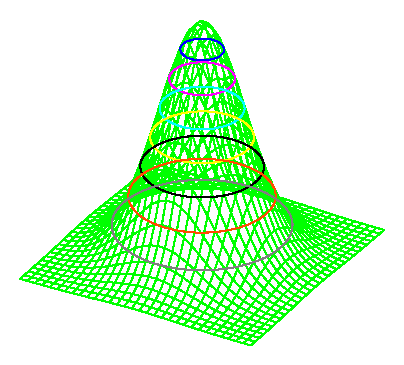
\includegraphics[width=\tw/4-5mm,clip=true]{../common/normxy_00.eps} &
  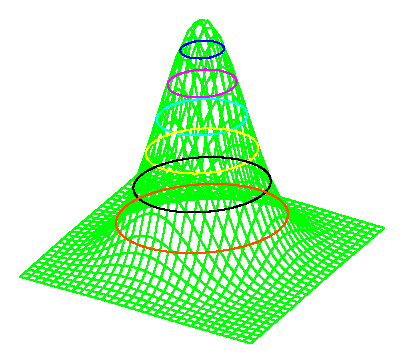
\includegraphics[width=\tw/4-5mm,clip=true]{../common/normxy_50.eps} &
  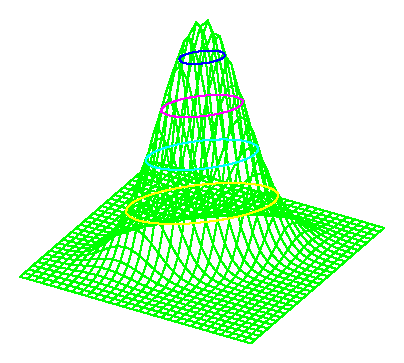
\includegraphics[width=\tw/4-5mm,clip=true]{../common/normxy_80.eps} &
  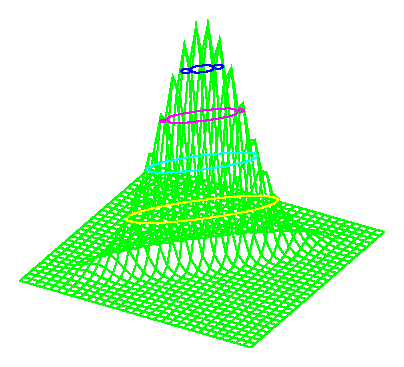
\includegraphics[width=\tw/4-5mm,clip=true]{../common/normxy_95.eps}
\end{tabular}
\caption{
  \fncte{Joint Gaussian distribution}s $\ppxy(x,y)$ with varying correlations
  \label{fig:psub_joint_gaussian}
  }
\end{figure}

%---------------------------------------
\begin{definition}[\fnctd{Joint Gaussian pdf}]
\footnote{
  \citerpgc{anderson1984}{21}{9780471889878}{\scshape Theorem 2.3.1},
  \citerpc{anderson1958}{14}{\textsection ``\scshape2.3 The Multivariate Normal Distribution"},
  \citerp{proakis}{49},
  \citerp{moon2000}{34}
  }
%---------------------------------------
\defbox{\begin{array}{rclD}
  \pp(x_1,x_2,\ldots,x_n)
    &\eqd& \ds\frac{1}{\sqrt{(2\pi)^n |\vM|}}
           \exp{-\frac{1}{2}(\vx-\pE\vx)^T\vM^{-1}(\vx-\pE\vx)}
    &      (Gaussian joint pdf)
    \\ \\
  \vx
    &\eqd& \left[\begin{array}{c}
             x_1    \\
             x_2    \\
             \vdots \\
             x_n
           \end{array}\right]
    \\
  \rvZ_k
    &\eqd& X_k - \pE X_k
    & (zero mean random variables)
    \\ \\
  \vM
    &\eqd& \brs{\begin{array}{cccc}
             \pE[\rvZ_1 \rvZ_1] & \pE[\rvZ_1 \rvZ_2] & \cdots & \pE[\rvZ_1 \rvZ_n]   \\
             \pE[\rvZ_2 \rvZ_1] & \pE[\rvZ_2 \rvZ_2] &        & \pE[\rvZ_2 \rvZ_n]   \\
             \vdots       & \vdots       & \ddots & \vdots         \\
             \pE[\rvZ_n \rvZ_1] & \pE[\rvZ_n \rvZ_2] & \cdots & \pE[\rvZ_n \rvZ_n]
           \end{array}}
    & (correlation matrix)
\end{array}}
\end{definition}


\begin{figure}[ht]
   \begin{center}
   \includegraphics[height=8cm, width=12cm, clip=]{../common/pdf_norm.eps}
   \end{center}
\caption{
  Gaussian pdf with $\mu=0$ and $\sigma\in[0.1,2]$.
  \label{fig:net_norm}
}
\end{figure}

%---------------------------------------
\begin{example}[1 variable joint Gaussian pdf]
%---------------------------------------
The \fnctd{Gaussian distribution} (or \fnctd{normal distribution} has pdf
\exbox{
  \ppx(x) \eqd \frac{1}{\sqrt{2\pi\sigma^2}}e^{\frac{-(x-\mu)^2}{2\sigma^2}}
  }

\begin{align*}
  t
    &= \arg_t \min_t
       \brs{
       \frac{1}{2}\int_t^\infty    \frac{1}{\sqrt{2\pi\sigma^2}}e^{\frac{-(x-\mu)^2}{2\sigma^2}} +
       \frac{1}{2}\int_{-\infty}^t \frac{1}{\sqrt{2\pi\sigma^2}}e^{\frac{-(x-\eta)^2}{2\sigma^2}}
       }
  \\&= \arg_t \brb{\pderiv{}{t}
       \brs{
       \frac{1}{2}\int_t^\infty    \frac{1}{\sqrt{2\pi\sigma^2}}e^{\frac{-(x-\mu)^2}{2\sigma^2}} +
       \frac{1}{2}\int_{-\infty}^t \frac{1}{\sqrt{2\pi\sigma^2}}e^{\frac{-(x-\eta)^2}{2\sigma^2}}
       }=0}
  \\&= \arg_t \brb{\frac{1}{2\sqrt{2\pi\sigma^2}}
       \brs{
       \pderiv{}{t}\int_t^\infty    e^{\frac{-(x-\mu)^2}{2\sigma^2}} +
       \pderiv{}{t}\int_{-\infty}^t e^{\frac{-(x-\eta)^2}{2\sigma^2}}
       }=0}
  \\&= \arg_t \brb{
       \brs{
       \brp{e^{\frac{-(\infty-\mu)^2}{2\sigma^2}}0 - e^{\frac{-(t-\mu)^2}{2\sigma^2}}1} +
       \brp{e^{\frac{-(t-\mu)^2}{2\sigma^2}}1 - e^{\frac{-(\infty-\mu)^2}{2\sigma^2}}0}
       }=0}
  \\&= \arg_t \brb{
       \brs{e^{\frac{-(t-\eta)^2}{2\sigma^2}}- e^{\frac{-(t-\mu)^2}{2\sigma^2}}}=0}
  \\&= \arg_t \brb{(t-\eta)^2=(t-\mu)^2}
  \\&= \frac{\mu+\eta}{2}
\end{align*}
\end{example}

%---------------------------------------
\begin{example}[2 variable joint Gaussian pdf]
\label{prop:prob_gaussian_xy}
%---------------------------------------
\exbox{\begin{array}{rc>{\ds}l}
  z_1 &\eqd& x_1 - \pE x_1 \\
  z_2 &\eqd& x_2 - \pE x_2 \\
  \abs{M} &\eqd& \abs{\pE[z_1 z_1]\pE[z_2 z_2]-\pE[z_1 z_2]\pE[z_1 z_2]}
  \\
  \pp(x_1,x_2) &\eqd&
    \frac{1}{2\pi \sqrt{\abs{M}}}
    \exp\left(
      \frac{z_1^2\pE[z_2z_2] - 2z_1z_2\pE[z_1z_2] + z_2^2\pE[z_1z_1]}
            {-2\abs{M}}
        \right)
\end{array}}
\end{example}

